\subsection{Assimétrica}

\begin{frame}{Criptografia assimétrica}
	\begin{figure}
		\begin{center}
			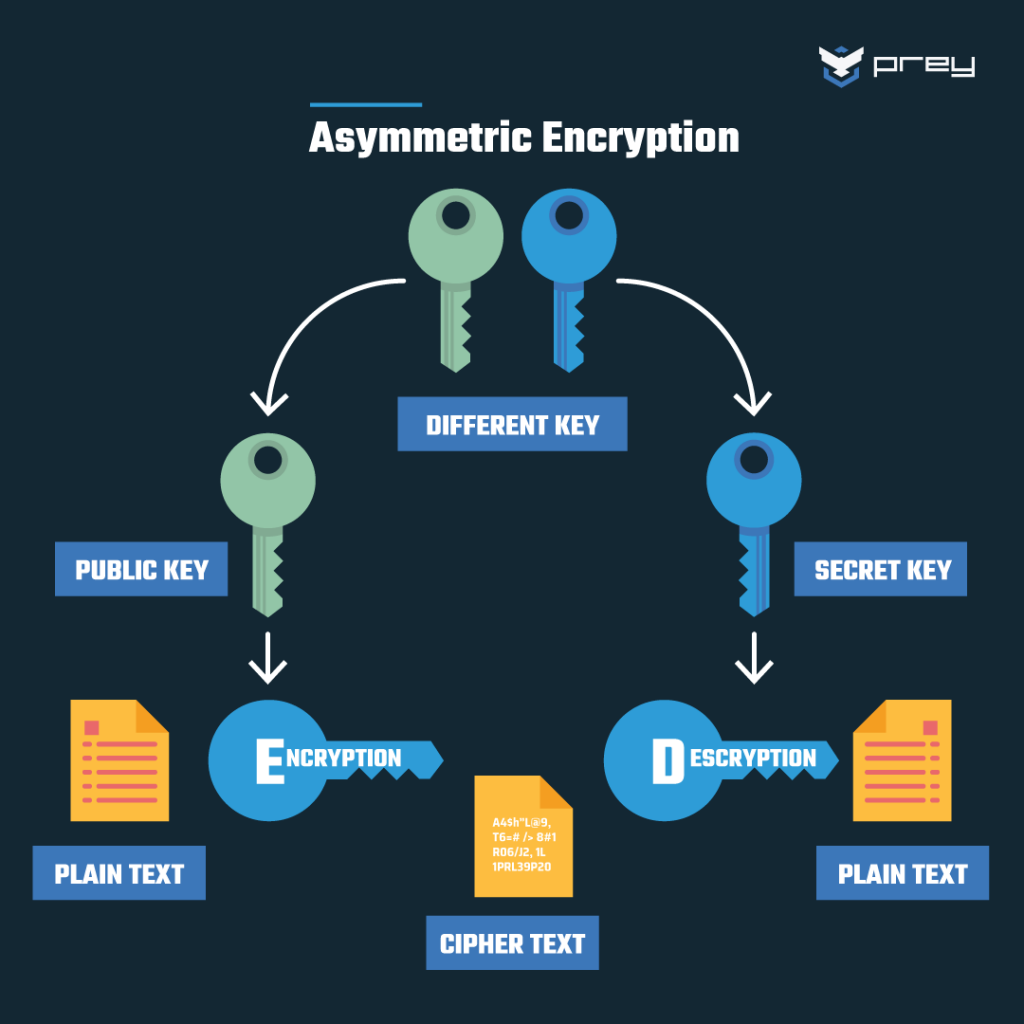
\includegraphics[
				width=0.95\textwidth,
				height=0.6\textwidth,
				keepaspectratio,
			]{Images/Asymmetric Encryption.png}
		\end{center}
		\footnotesize
		Fonte: \hyperlink{https://findwithinformationsecurity.blogspot.com/2024/05/symmetric-ciphers.html}{With Information Security}
	\end{figure}
\end{frame}

\begin{frame}{Ponta a Ponta}
	\begin{figure}
		\begin{center}
			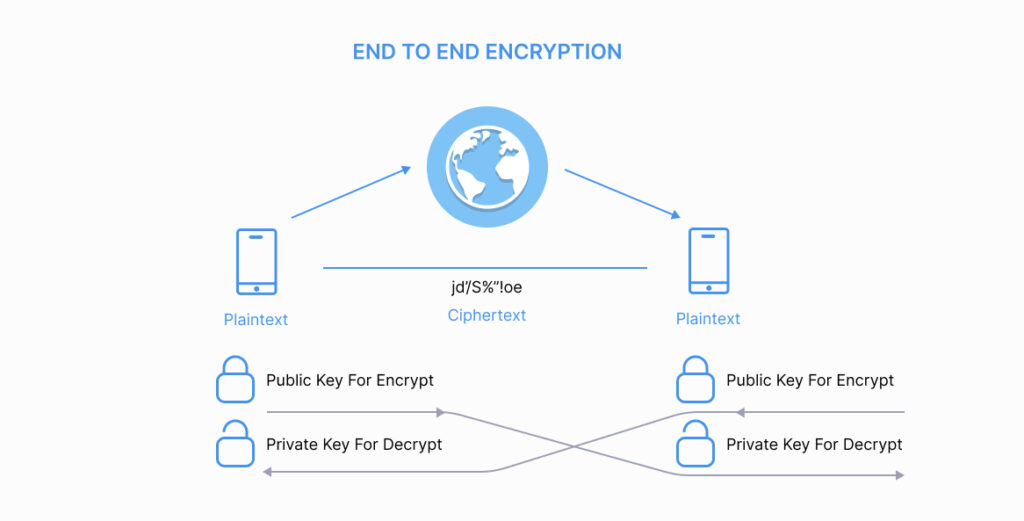
\includegraphics[
				width=0.95\textwidth,
				height=0.6\textwidth,
				keepaspectratio,
			]{Images/End to end encryption.jpg}
		\end{center}
		\footnotesize
		Fonte: \hyperlink{https://helenix.com/blog/end-to-end-encryption-ee2e/}{Helenix}
	\end{figure}
\end{frame}

\begin{frame}{Ponta a Ponta}
	\begin{figure}
		\begin{center}
			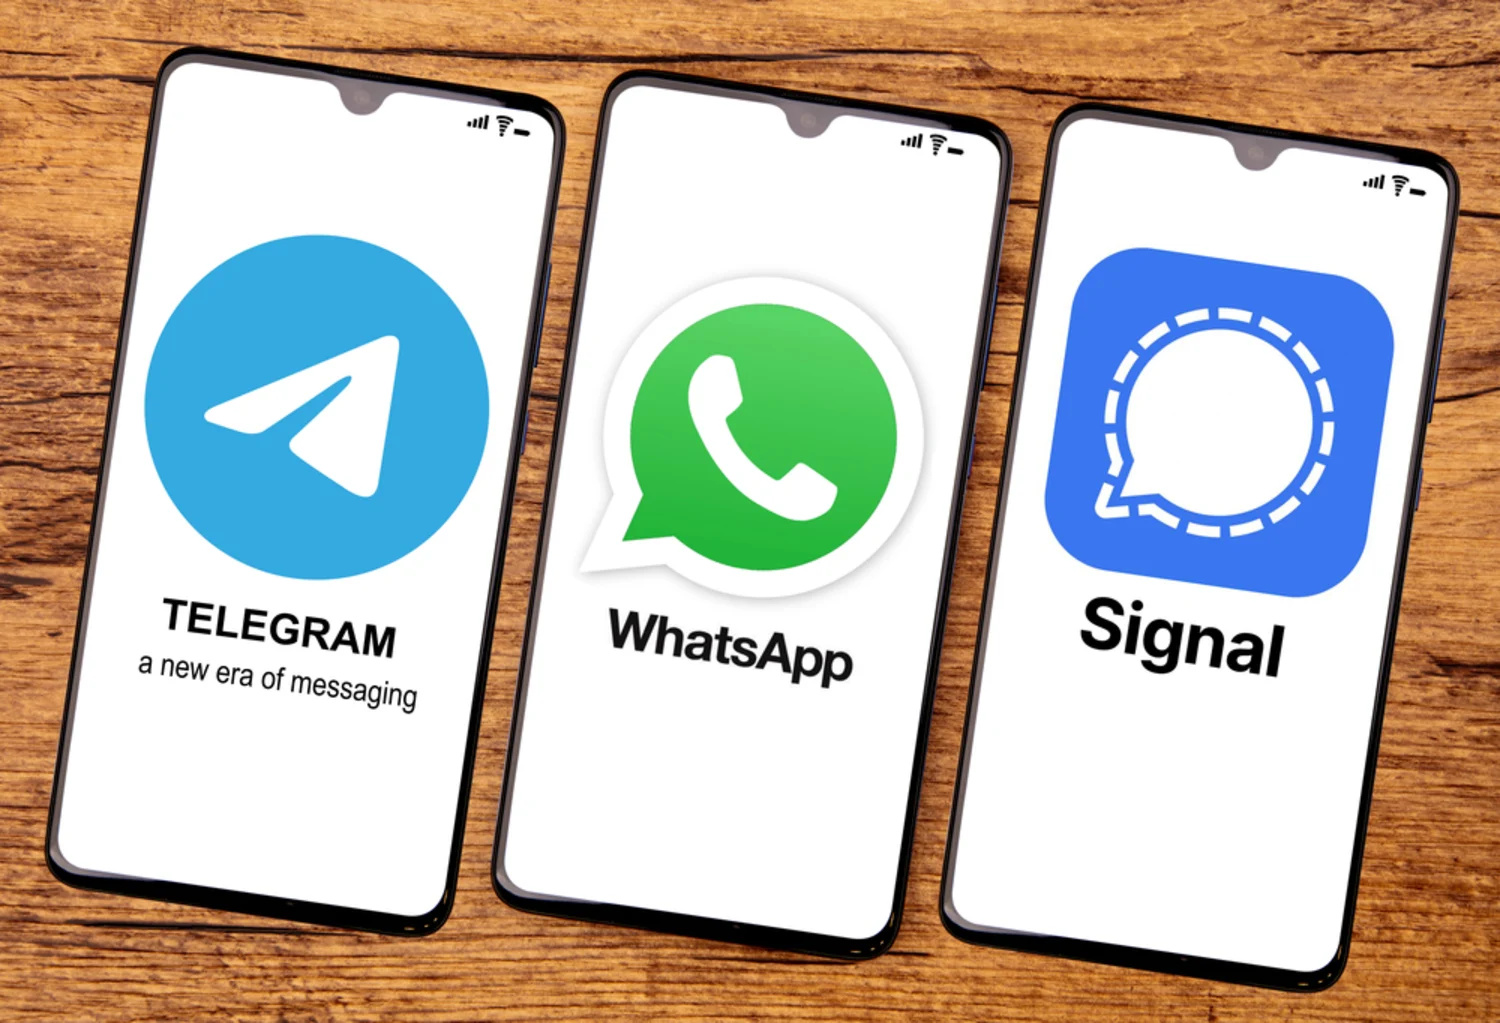
\includegraphics[
				width=0.95\textwidth,
				height=0.6\textwidth,
				keepaspectratio,
			]{Images/WhatsApp vs Signal vs Telegram.jpg}
		\end{center}
	\end{figure}
\end{frame}

